\documentclass[12pt,letterpaper]{article}

\usepackage{amsmath, amsthm}
\usepackage{graphicx,hyperref}
\usepackage{microtype, parskip}
\usepackage[numbers,sort&compress]{natbib}
\usepackage{lineno}
\usepackage{docmute}
\usepackage[font=small]{caption}
\usepackage{subcaption, multirow, morefloats}
\usepackage{wrapfig}
\usepackage{titlesec}
\usepackage{authblk, attrib, fullpage}
\usepackage{lineno}

\frenchspacing

\captionsetup[subfigure]{position = top, labelfont = bf, textfont = normalfont, singlelinecheck = off, justification = raggedright}

\begin{document}
\section{Results}

\begin{figure}[ht]
  \centering
  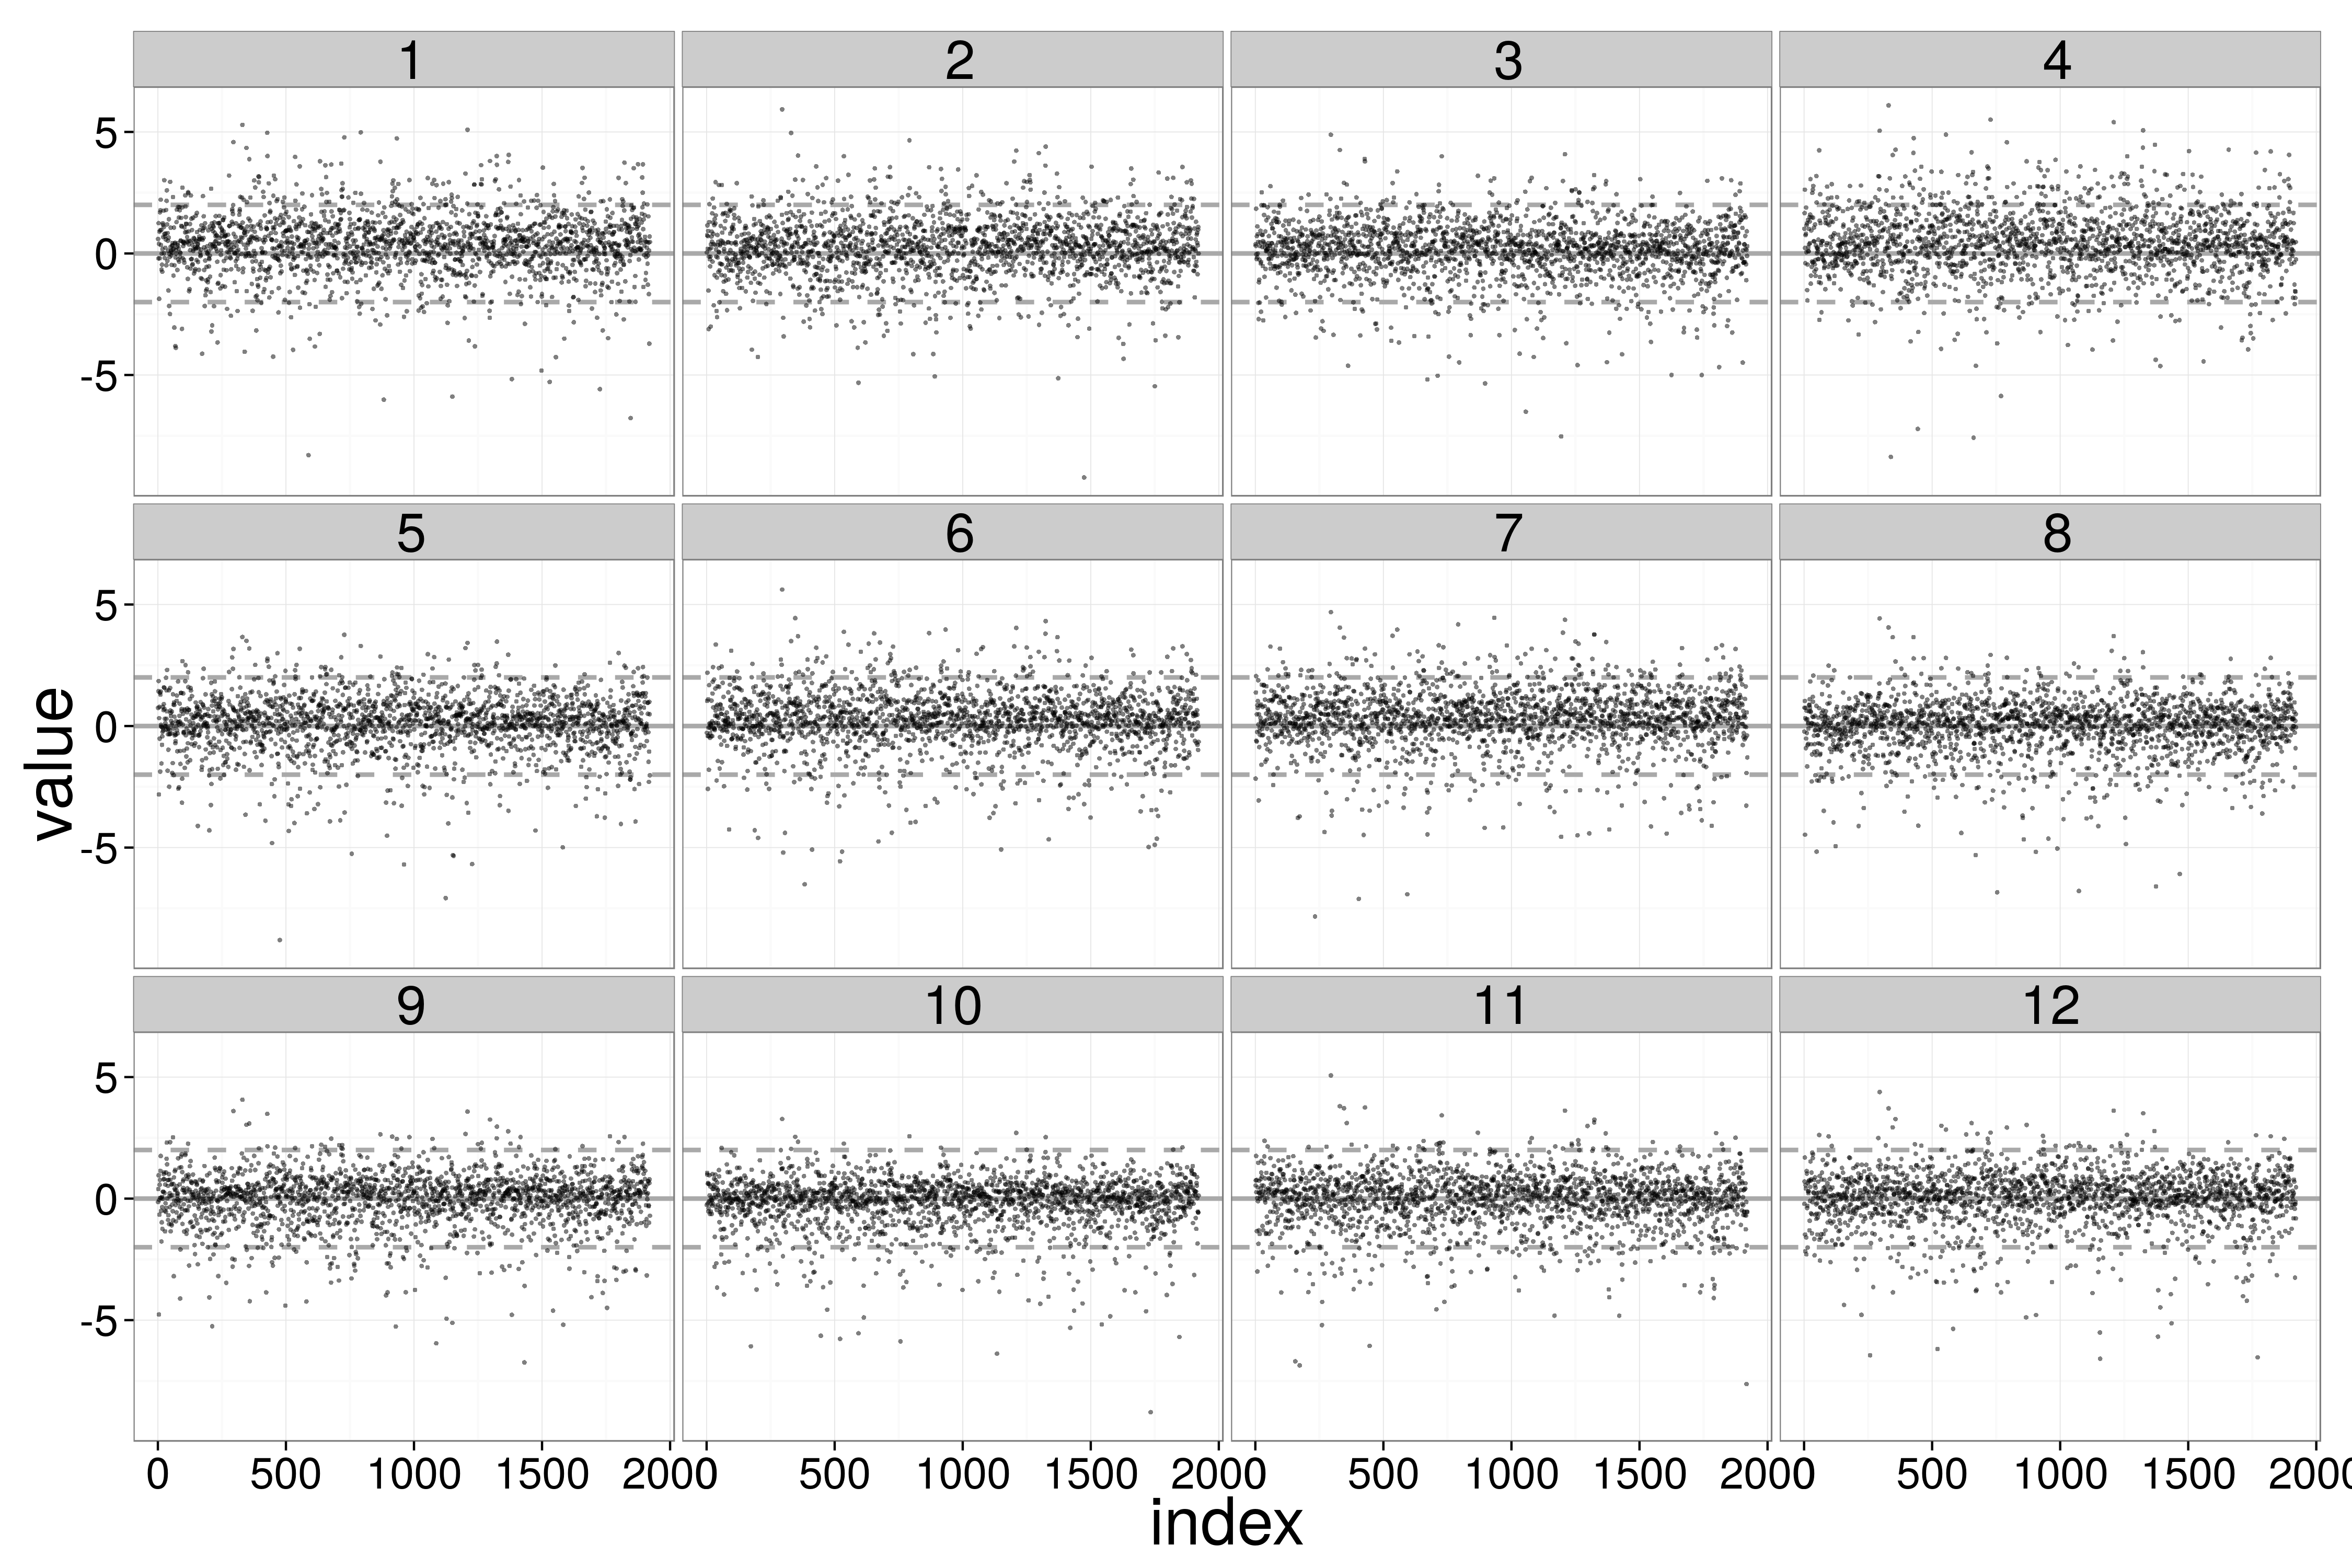
\includegraphics[height = 0.5\textheight, width = \textwidth, keepaspectratio = true]{figure/residual_plot}
  \caption{Deviance residuals from the fitted survival model. Each graph depicts the residuals from single draws from the posteriors distributions of all estimated parameters. Positive values indicate an under estimate of the observed duration, while negative values indicate an over estimate of the observed duration. Twelve difference examples are provided here to indicate the lack of individual observation based biases.}
  \label{fig:ppc_res}
\end{figure}

\begin{figure}[ht]
  \centering
  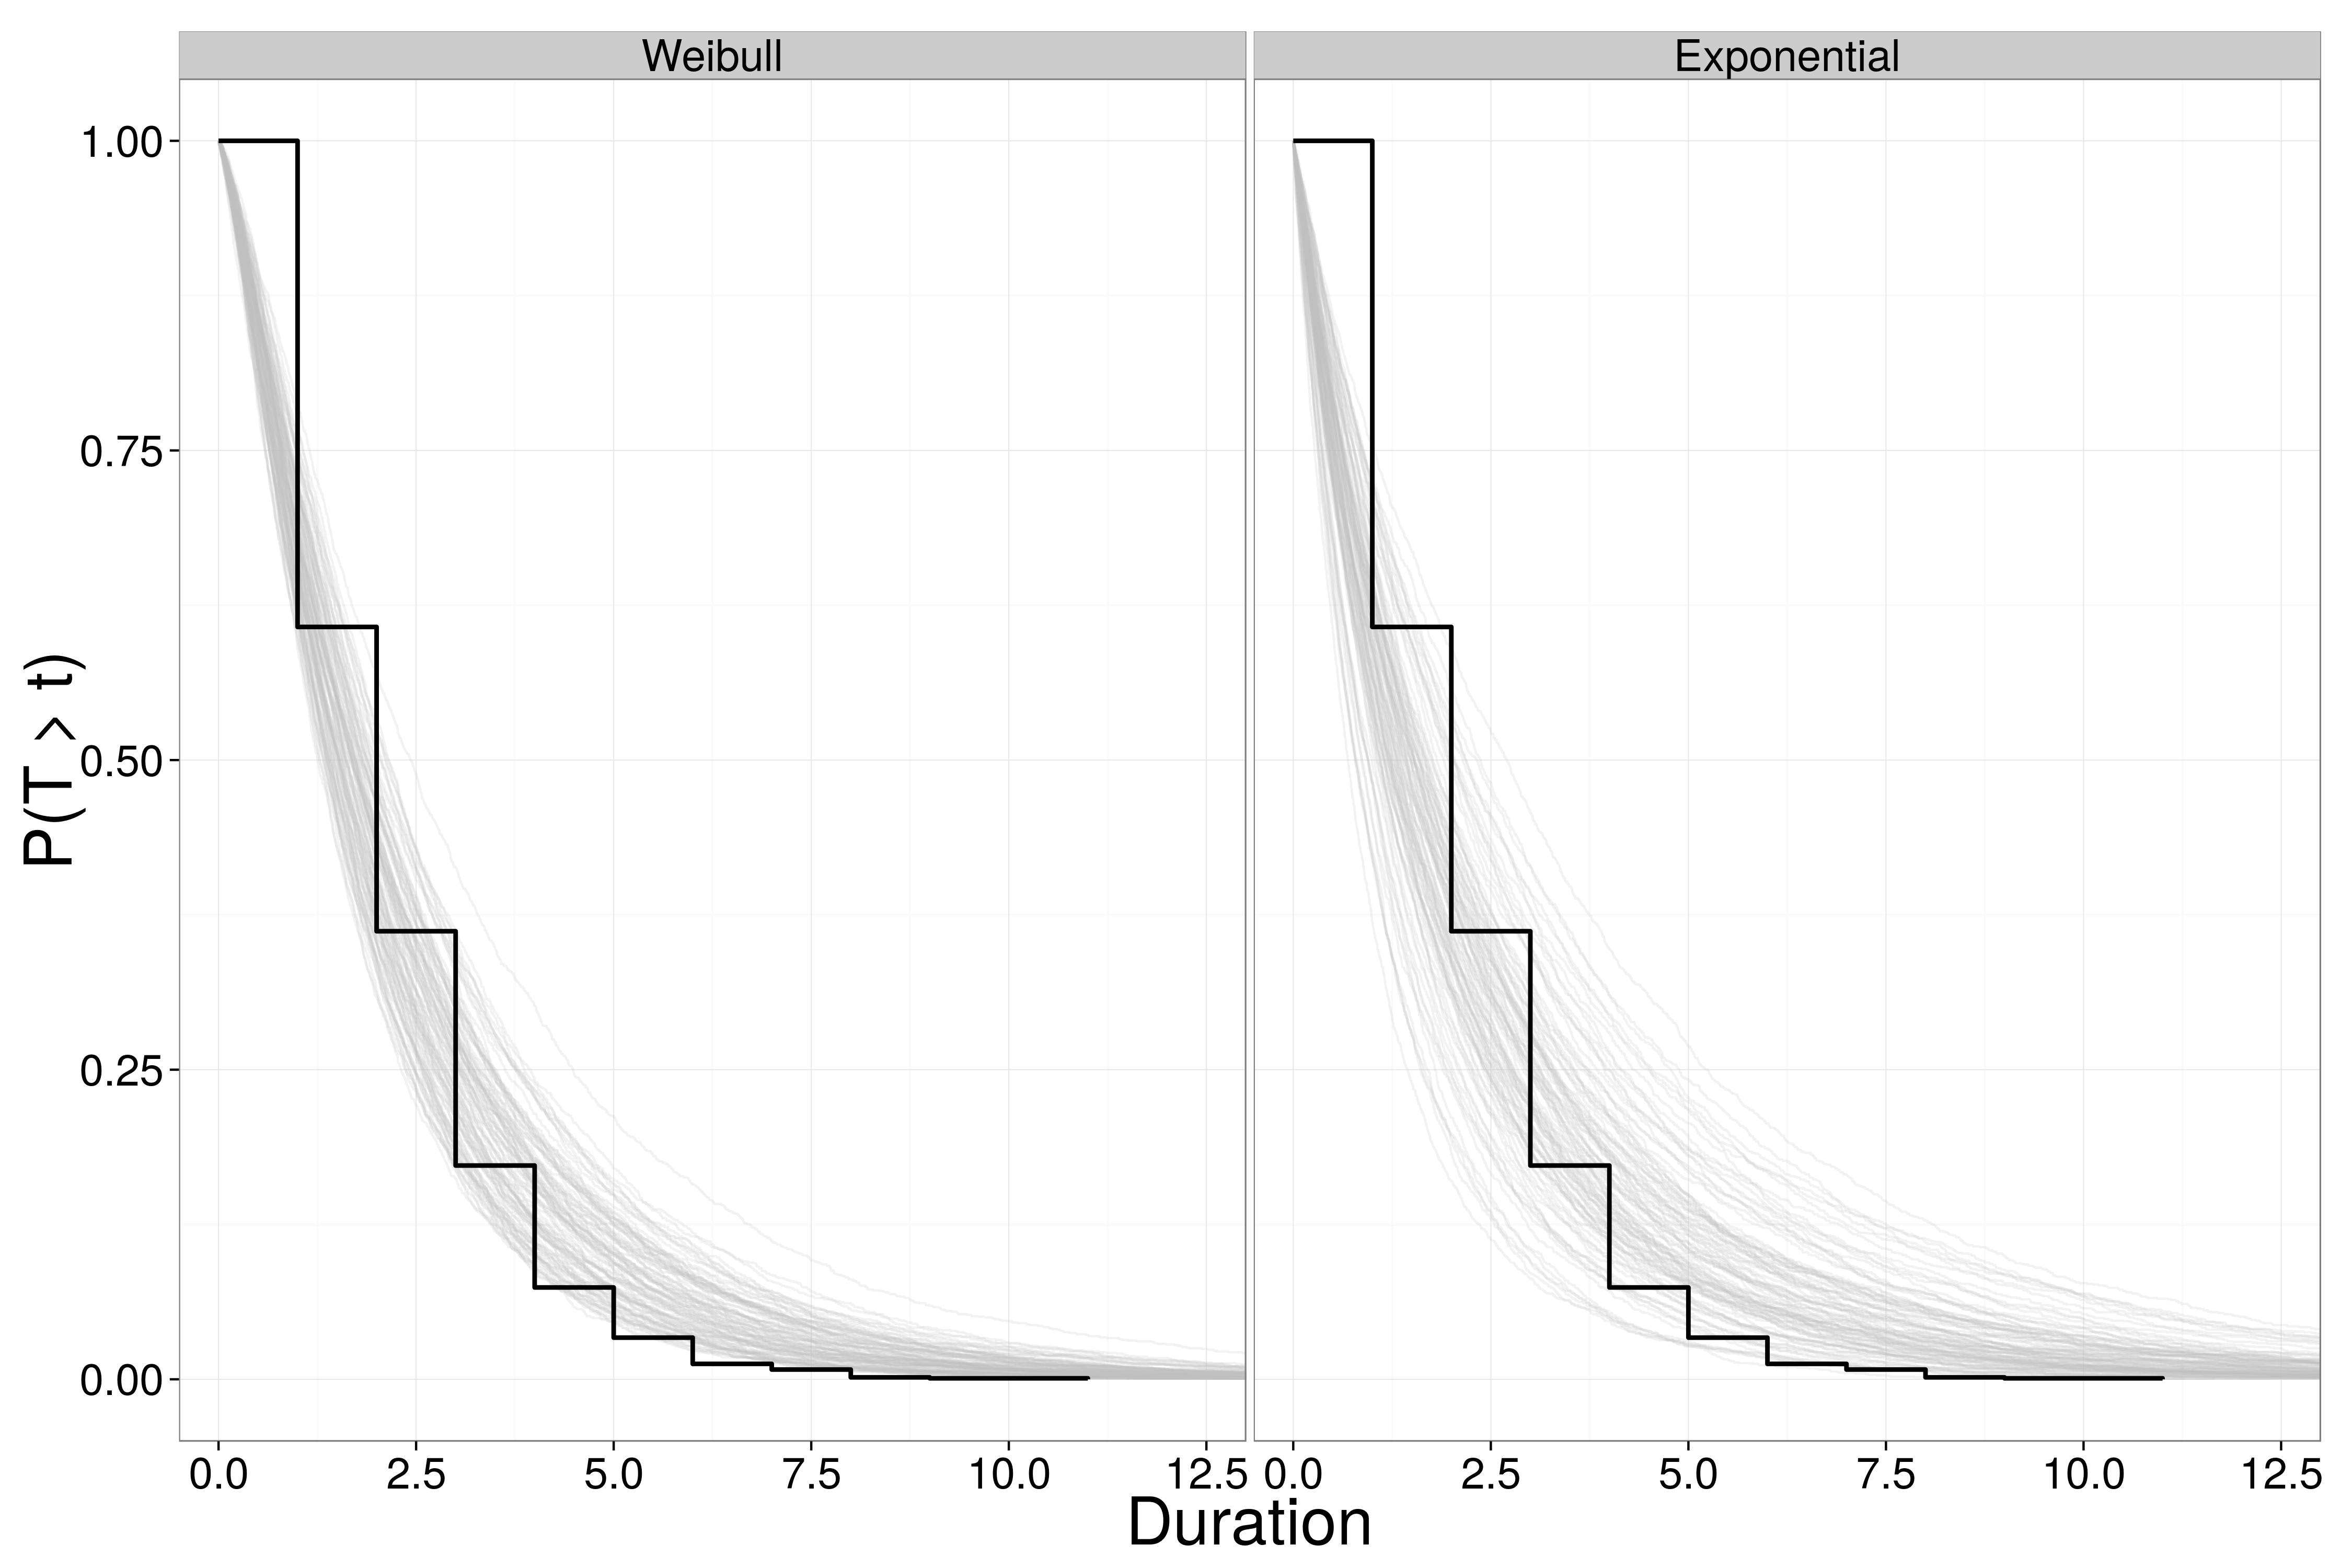
\includegraphics[height = 0.5\textheight, width = \textwidth, keepaspectratio = true]{figure/survival_function}
  \caption{Comparison between K-M estimate of survival function (black) from the observed versus K-M estimates from 100 simulated data sets using the fitted model (dark grey). Simulated data sets were generated by drawing parameter values randomly from their estimated posteriors and using the observed covariate information to estimate durations for all the observed species. On the left are the results from the full survival model (Fig. \ref{fig:model_diagram}), while on the right are the results from a simplified model where duration follows an exponential distribution and there is no phylogenetic effect.}
  \label{fig:ppc_surv}
\end{figure}

\begin{figure}[ht]
  \centering
  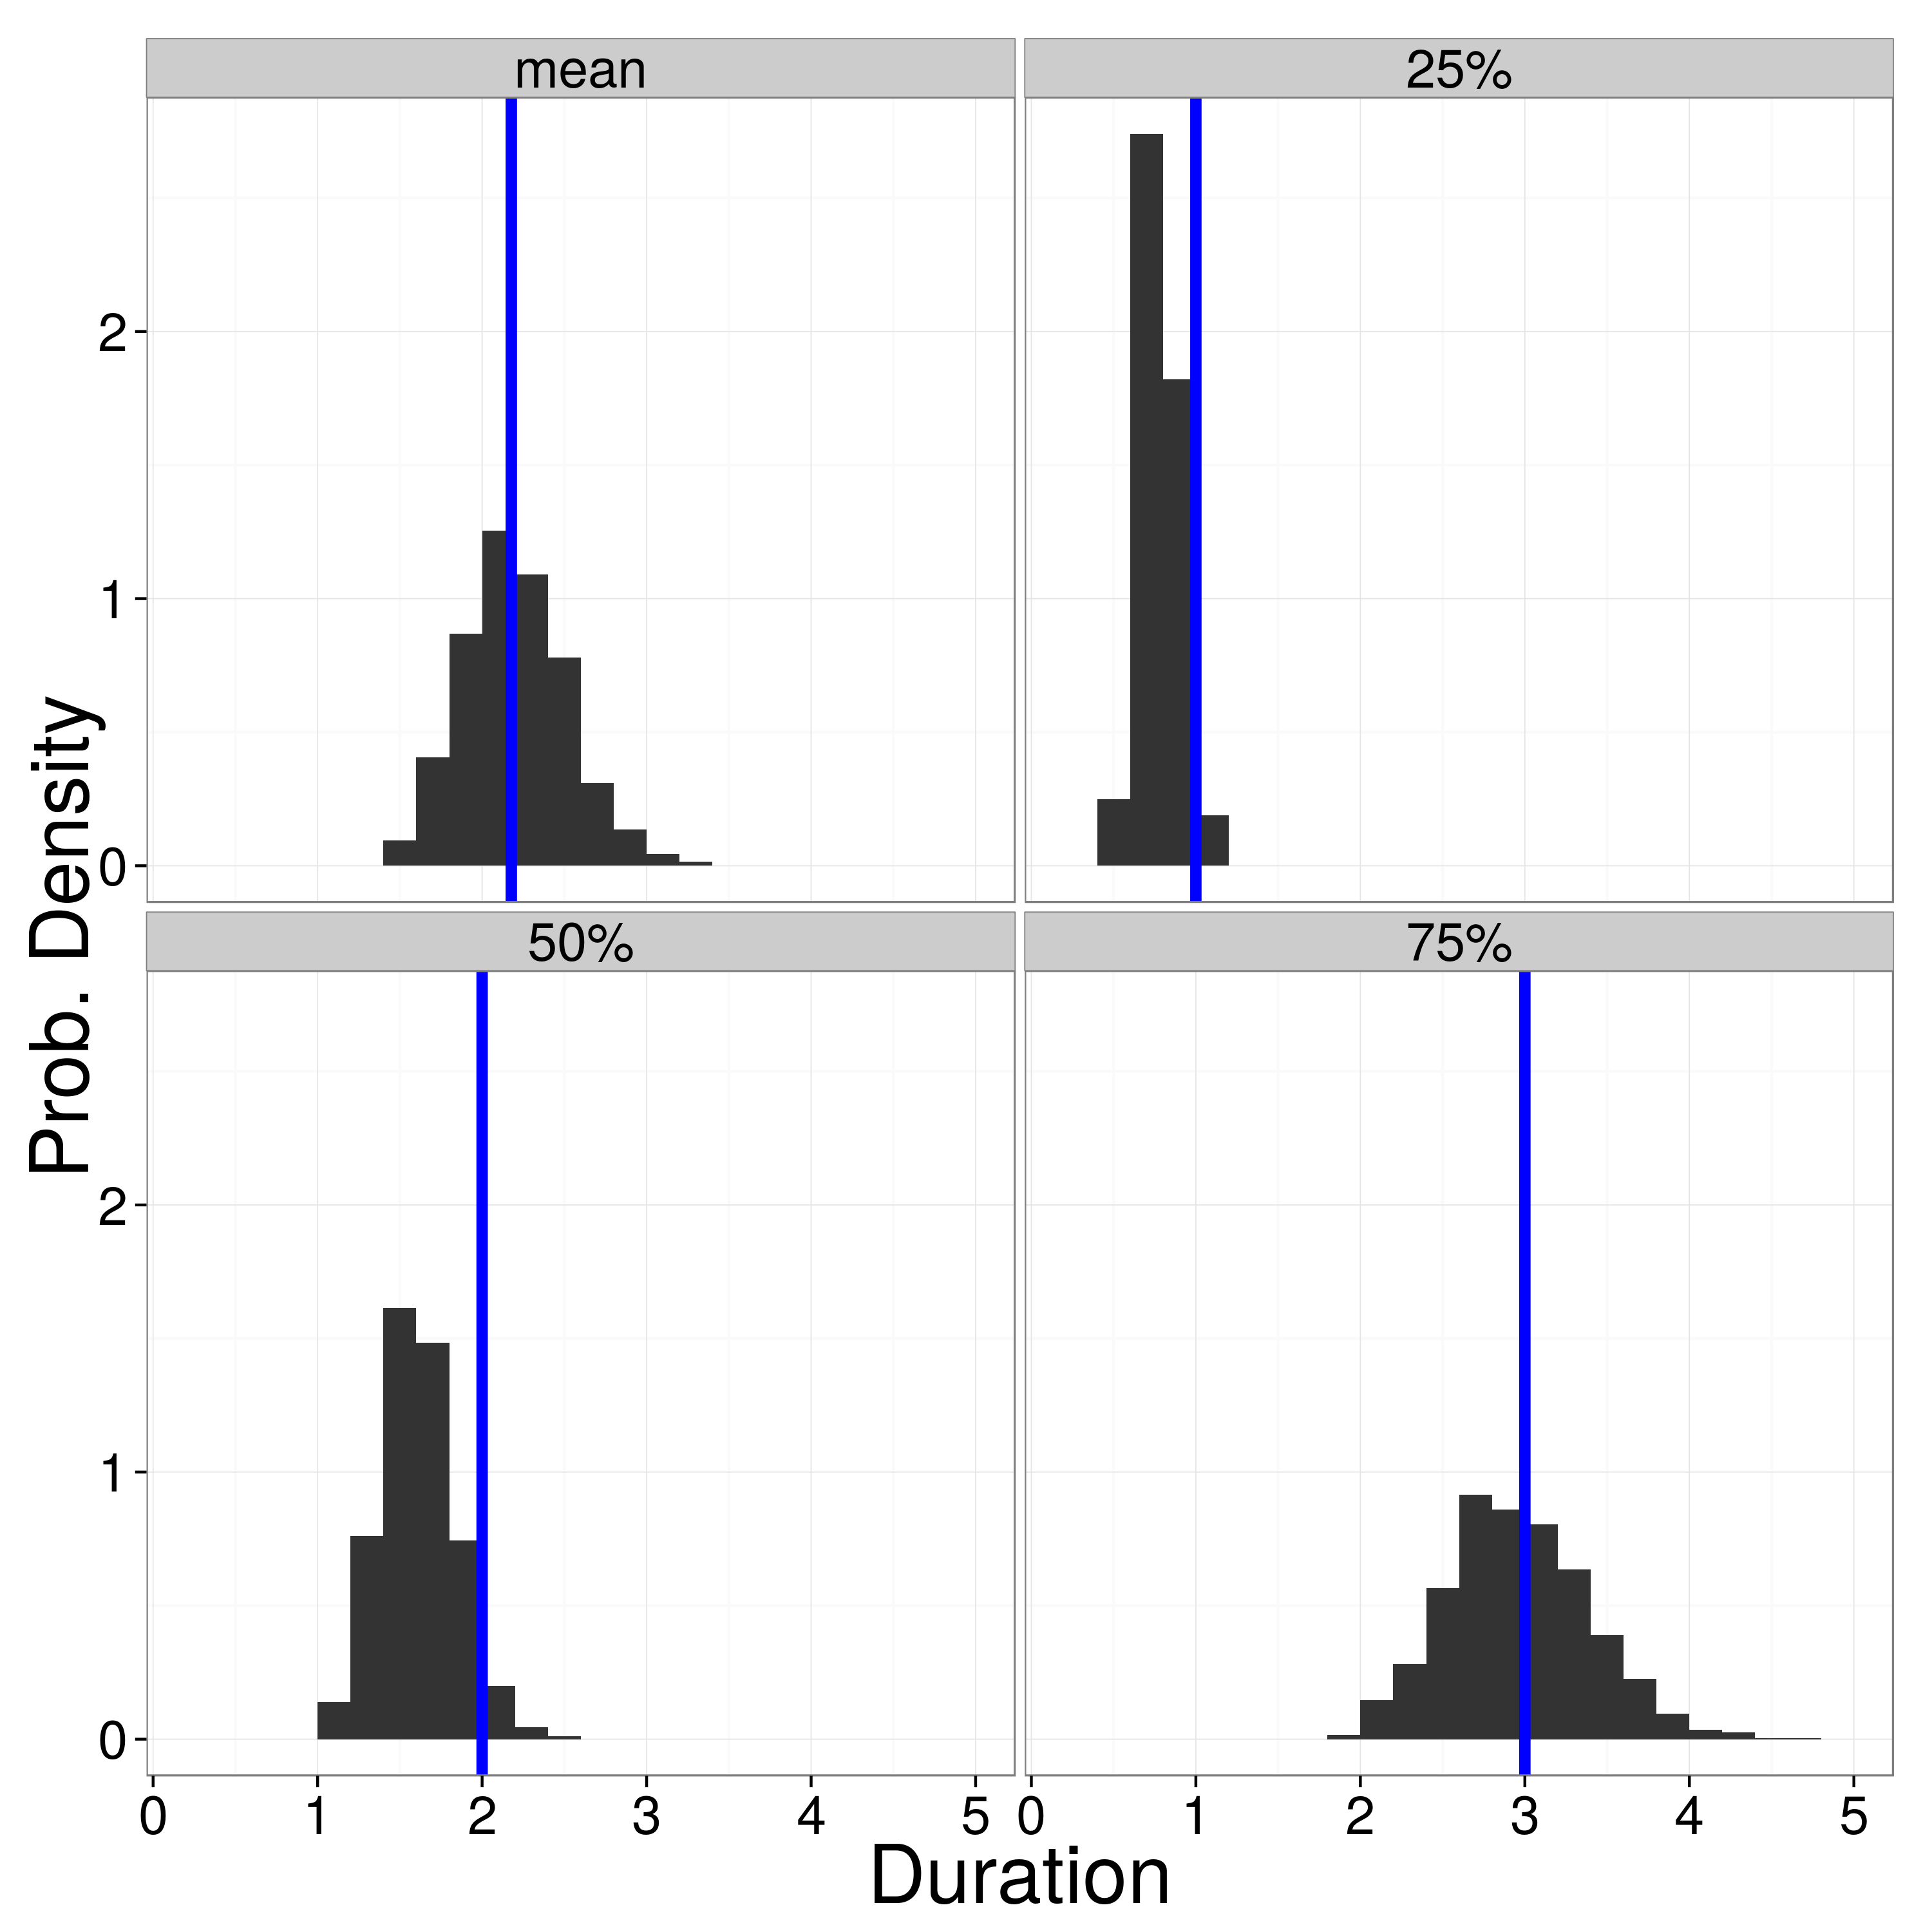
\includegraphics[height = 0.5\textheight, width = \textwidth, keepaspectratio = true]{figure/quant_ppc}
  \caption{The results of additional posterior predictive checks for four summaries of the observed durations, as labeled. Blue vertical indicate the observed value. None of the observed are significantly different from the posterior predictive distributions.}
  \label{fig:ppc_quant}
\end{figure}

% Model deficiencies.

% fit summary
%   graph: with each individual species level effect
%   or
%   table: with summaries of the effects and \hat{R} values THIS

\begin{figure}[ht]
  \centering
  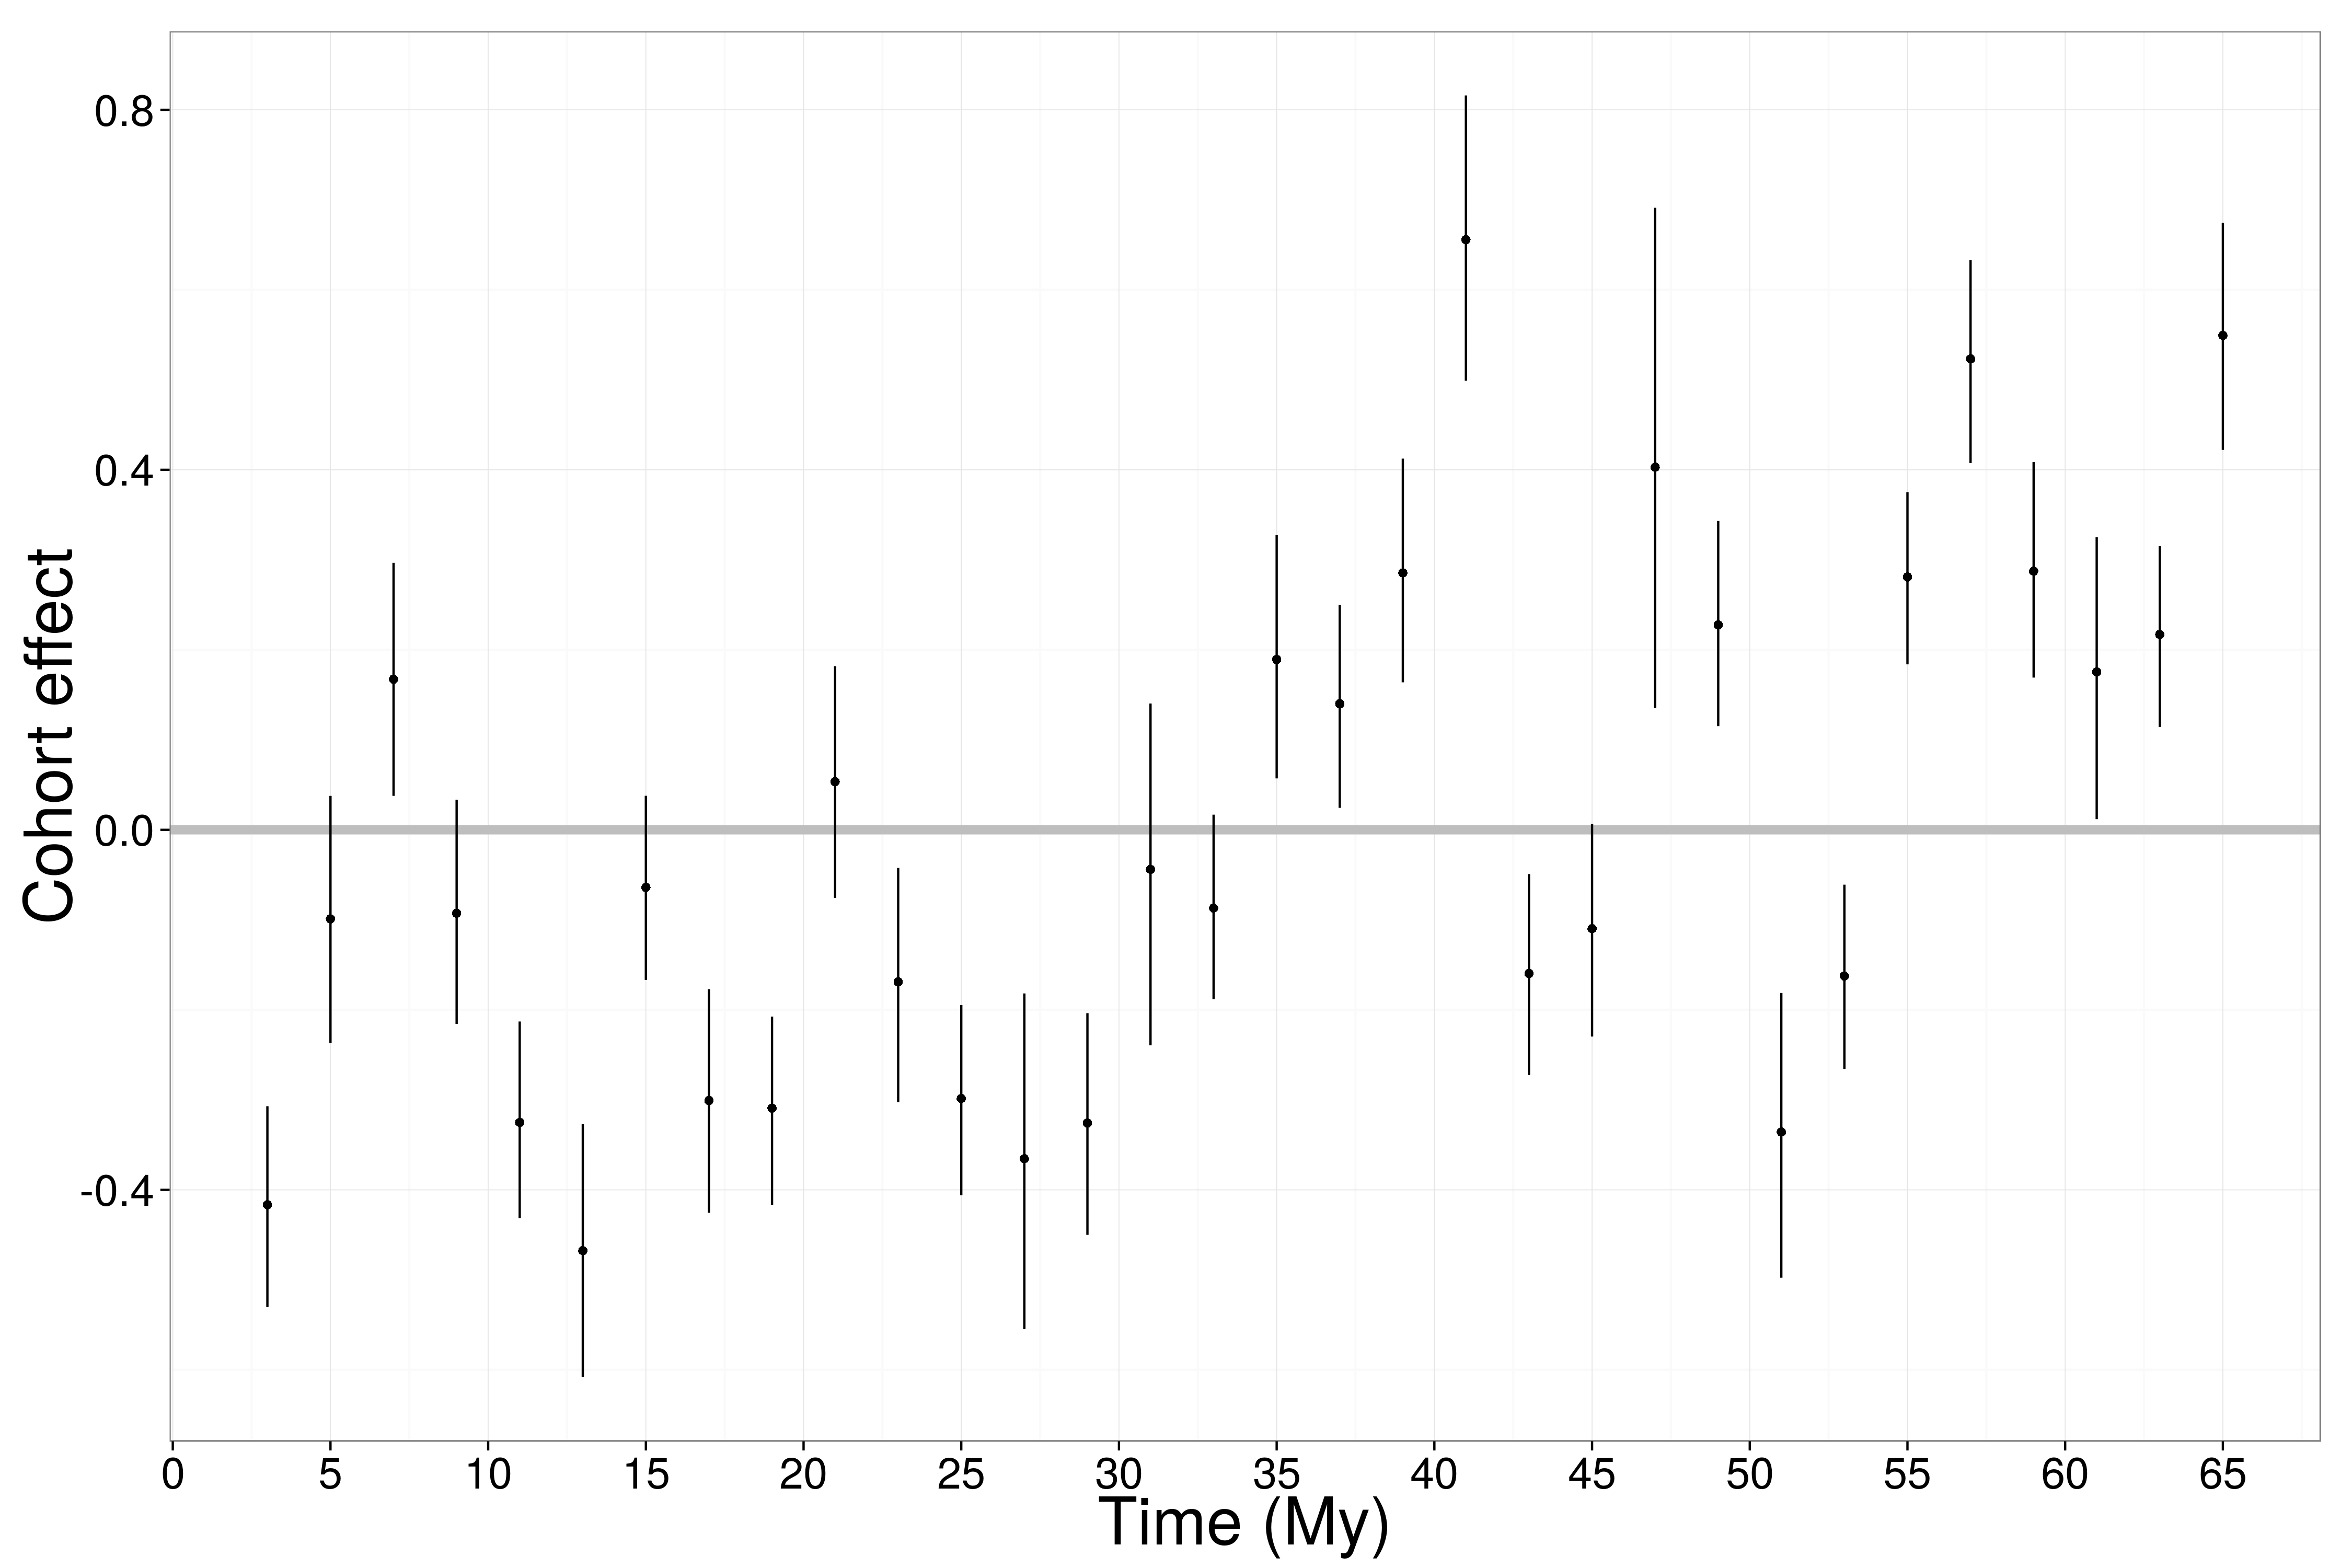
\includegraphics[height = 0.5\textheight, width = \textwidth, keepaspectratio = true]{figure/cohort_est}
  \caption{Summaries of estimated individual cohort effect posteriors. Depicted are medians and 80\% credible intervals of the estimated posterior distributions. High values correspond to shorter species durations while lower values correspond to greater species durations compared to the mean duration. Lines are placed at the middle of the 2 My origination cohorts.}
  \label{fig:eff_cohort}
\end{figure}

\begin{figure}[ht]
  \centering
  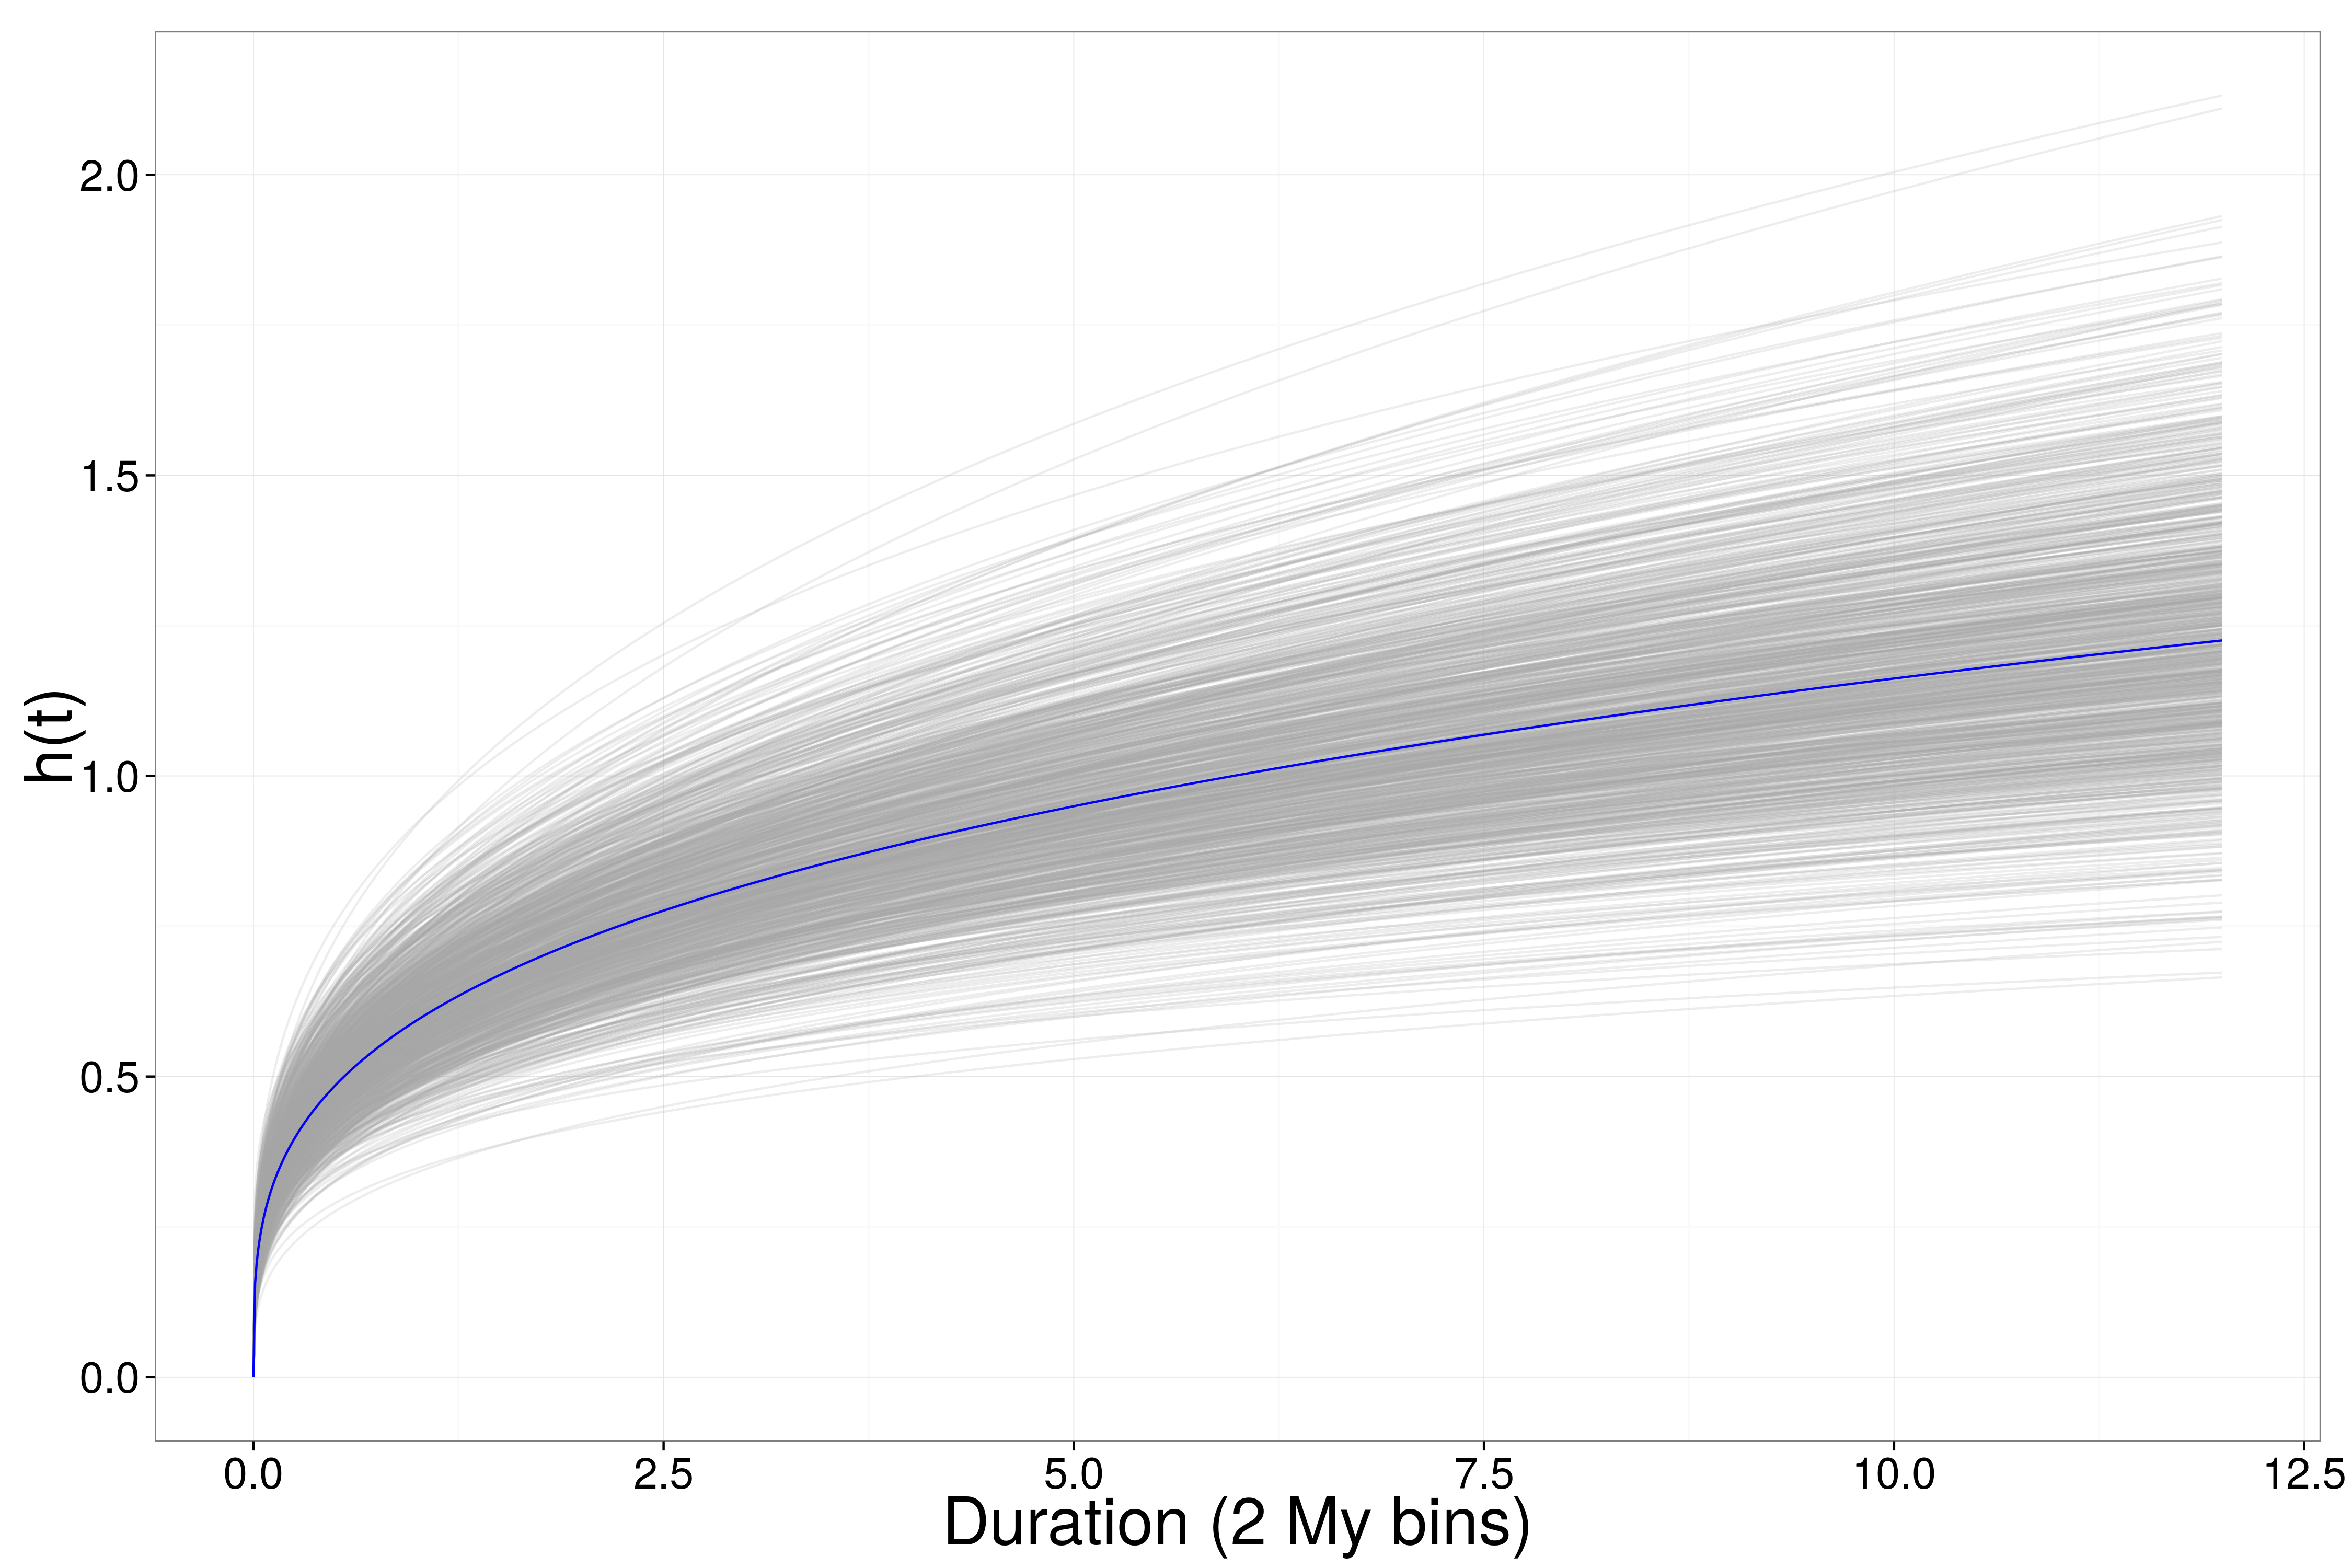
\includegraphics[height = 0.5\textheight, width = \textwidth, keepaspectratio = true]{figure/haz_est}
  \caption{100 estimates of the hazard function (\(h(t\)) for the observed species mean (grey), along with the median estimated hazard function. \(h(t)\) is an estimate of the number of extinctions that occur given an amount of time, \(t\). Hazard functions were estimated from random draws from the estimated posterior distributions and evaluated with all covariate information set to 0, which corresponds to the expected duration of the mean species.}
  \label{fig:haz}
\end{figure}

\begin{figure}[ht]
  \centering
  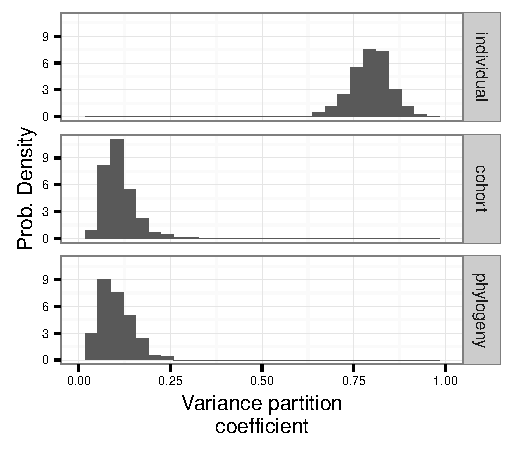
\includegraphics[height = 0.5\textheight, width = \textwidth, keepaspectratio = true]{figure/variance_est}
  \caption{Estimates of the variance partitioning coefficients for the three different sources of variance: species, cohort, and phylogeny. Higher values correspond to greater contribution to total variance. Each of the estimates is a distribution of 1000 approximating simulations due to the models non-normality.}
  \label{fig:vpc}
\end{figure}




\end{document}
